\newpage
\part{Modification of terrain (terraforming) assessment} \label{part:mt}

\section{Introduction to the ModifyTerrain module} \label{sec:mtintro}
The \textit{ModifyTerrain} module can remodel the terrain DEM according to widen (berm setback) and grading threshold values to enable plantings. Moreover, the module quantifies mass movement volumes by comparing an initial DEM with a modified DEM. Modified DEMs can be automatically generated for widen and grading features based on maximum lifepsan maps or manually created for other framework features or any terrain modification. The module produces spreadsheets containing reach-wise volume differences (excavation and fill), modified raster DEMs, \texttt{mxd}-layouts and \texttt{pdf}-maps. This chapter explains the module application in the following sections:\\
\begin{tabular}{l L{0.9\textwidth}}
\multicolumn{2}{l}{}\\
Section~\ref{sec:mtquick}: & Quick Guide to the application of the GUI with descriptions of input requirements and output descriptions.\\
Section~\ref{sec:mtprin}:  & Descriptions of outputs and procedures for half-automated pdf-map generation.\\
Section~\ref{sec:mtcode}:  & Detailed explanations of coding conventions with descriptions of extension possibilities.\\
\multicolumn{2}{l}{}\\
\end{tabular}

Please note that an \textit{ArcGIS} \texttt{3D} extension is required for running this module.

\section{Quick GUIde to terrain assessment} \label{sec:mtquick}
\subsection{Main window set-up and run} 
The GUI start-up takes a couple of seconds because the module updates reach information from a spreadsheet. Fig.~\ref{fig:gui_start_mt} shows the \textit{ModifyTerrain} GUI at start-up. First, the module requires the choice of a feature set from the dropdown menu, which limits to ``CUSTOM'', ``Widen'' and ``Grading''. Second, a \texttt{condition} (exactly four characters, corresponding to Sec.~\ref{sec:input}) needs to be defined, which requires a click on the ``Verify'' button to update the windows. This behavior is different from the \textit{LifespanDesign} and \textit{MaxLifespan} modules.
\begin{figure}[hbt]
	\begin{center}
	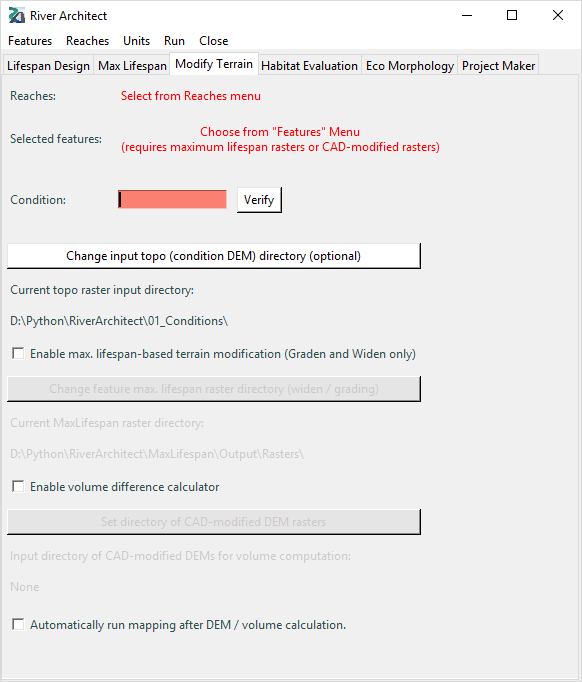
\includegraphics[width=0.7\columnwidth]{gui_start_mt.PNG} % Example image
	\caption{GUI start up window. \label{fig:gui_start_mt}}
	\end{center}
\end{figure}

\subsection{Input: Set initial DEM input folder}
For terrain modifications, the module requires an input topo (DEM), which it looks up in the \texttt{.../RiverArchit ect/LifespanDesign/Input/\textit{condition}/} directory by default. The input directory can be modified by clicking on the ``Change input topo (condition DEM) directory (optional)'' button. Note that the input folder needs to contain a GRID-type DEM raster with the name \texttt{dem}; other raster names are not recognized and the input \texttt{dem} is crucial for any operation of the module.

\subsection{Input: Set Reaches} \label{sec:mtsetreaches}
A particularity of this module is that it enables running analysis for specific river reaches, which can be renamed and the reach extents can be modified. By default, the module analyzes all reaches which are defined in a spreadsheet stored in \texttt{/ModifyTerrain/.templates/computation{\myUnderscore}extents.xlsx}. This spreadsheet, shown in Fig.~\ref{fig:computation_extents_illu}, can be opened by clicking on the \texttt{Modify Reaches} dropdown menu and then ``\texttt{DEFINE REACHES}''.

\begin{figure}[hbt]
	\begin{center}
	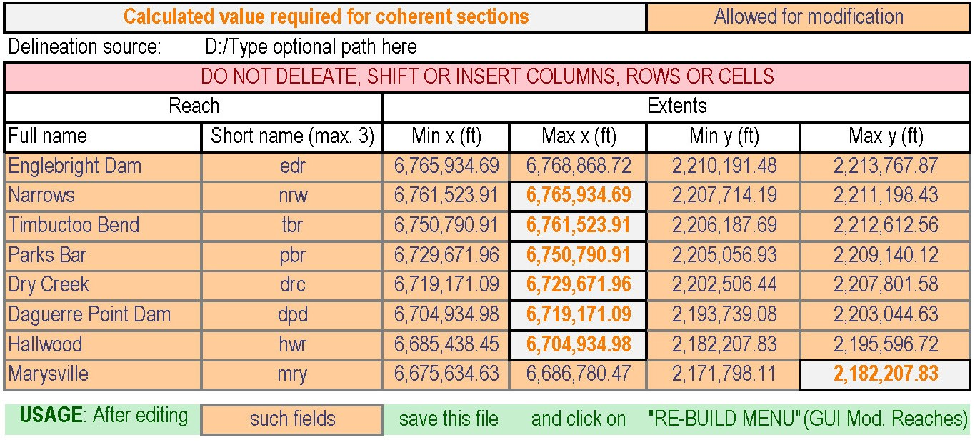
\includegraphics[width=0.95\columnwidth]{computation_extents_illu.pdf} % Example image
	\caption{Spreadsheet with reach definitions (stored in \texttt{ModifyTerrain/.templates/computation{\myUnderscore}extents.xlsx}). \label{fig:computation_extents_illu}}
	\end{center}
\end{figure}

The workbook enables the definition of up to eight reach names and the extents. The extents need to correspond to the input DEM coordinate and unit system types. In the example of Fig.~\ref{fig:computation_extents_illu}, the unit system is \texttt{GRS{\myUnderscore}1980{\myUnderscore}Lambert{\myUnderscore}Con formal{\myUnderscore}Conic} with the linear unit of \texttt{Foot{\myUnderscore}US}. If the reaches 00 to 07 align from the East to the West, the \texttt{Max x} value of a reach corresponds to the \texttt{Min x} value of the next upstream reach. If a is situated in the south of an upstream reach, its \texttt{Max y} value corresponds to the \texttt{Min y} value of the upstream reach. These gap-less transitions enable consistent mapping of DEM differences and excavation/fill volume calculations.\\

After editing, saving and closing the spreadsheet, the GUI window can be updated by clicking on the \texttt{Modify Reaches} dropdown menu and then ``\texttt{RE-BUILD MENU}''. Whatever name is stored in the spreadsheet, the module uses internal identifiers that point at the rows in the spreadsheet, and therefore, output rasters are enumerated with tags \texttt{r00}, \texttt{r01}, ... \texttt{r07}.\\

All reaches can be deselected by clicking on ``\texttt{CLEAR ALL}'' to add particular reaches only. If more than five reaches are selected, the GUI truncates the list and displays \texttt{Many / All}.

\subsection{Input: CUSTOM DEM options}\label{sec:mtcustdem}
If the ``CUSTOM: Use CAD-modified DEM'' feature was selected, the \texttt{Enable volume difference calcu lator} check box is auto-selected as required module operation. In addition, the check box \texttt{Automatically run mapping after DEM / volume calculation} can be selected to map volume differences between the initial DEM and the customary modified DEM. By default, the module looks for a modified DEM in the folder \texttt{ModifyTerrain/Input/DEM/\textit{condition}/} and the modified DEM needs to have either the string \texttt{dem} or a feature shortname (Sec.~\ref{sec:featoverview}) in its name for getting recognized. The directory of the modified DEM can be changed by clicking on the \texttt{Set directory of CAD-modified DEM rasters} button, but the \textbf{name convention (raster DEM name contains \texttt{dem} or feature shortname) always needs to be respected}. Refer to Sec.~\ref{sec:mtvoldiff} for more information on volume difference (fill/excavate) calculation with customary DEMs.

\subsection{Input: Widen and Grading options}\label{sec:mtdemmod}
The ``Widen'' and ``Grading'' features use the maximum required distance to the groundwater table, which is admissible for plantings. These threshold values are defined in the \textit{LifespanDesign} modules spreadsheet \texttt{RiverArchit ect/LifespanDesign/Input/.templates/threshold{\myUnderscore}values.xlsx} (see explanations in Sec.~\ref{sec:modthresh}). If the \texttt{Enable max. lifespan raster-based terrain modification (Grading and Widen only)}\\ check box is selected, the module provides the option \texttt{Run: DEM Modification} to apply the threshold values defined in the cells \texttt{J6:M6} for lowering the terrain where maximum lifepsan rasters indicate that widening and grading are most pertinent. Thus, the prior run of the \textit{MaxLifespan} module is required to enable \textit{ModifyTerrain} reading rasters containing the keywords \texttt{grade} or \texttt{widen} from the folder \texttt{RiverArchitect/MaxLifespan/Output/Rasters/\textit{condition}/}. Moreover, a depth to groundwater table raster (GRID format) with the name \texttt{d2w} is required in the directory \texttt{RiverArchitect/LifespanDesign/Input/\textit{condition}/}.\\
The directory of maximum lifespan and depth to groundwater rasters can be modified by clicking on the \texttt{Change feature max. lifespan raster directory (widen/grading)} button, but there need to be rasters in the defined folders which contain the keywords \texttt{grade} or \texttt{widen} in their name. The DEM modification auto-selects the \texttt{Enable volume difference calculator} check box. Please note that the volume calculator is executed after the automated terrain modification, even if the check box is deselected.\\
Selecting the check box \texttt{Automatically run mapping after DEM / volume calculation} enables mapping of volume differences between the initial DEM and the customary modified DEM, as well as mapping of the modified DEMs after widening and grading.

\subsection{Input: Prepare mapping layouts}\label{sec:mtlyt}

The Run: Map Maker uses layout files (\texttt{.mxd}) stored in the directory \texttt{ModifyTerrain/Input/Layouts/\textit{condition}/}. Template layout files are provided in \texttt{ModifyTerrain/Input/Layouts/Templates/} and need to be manually copied and adapted to the \texttt{\textit{condition}}:
\begin{enumerate}
	\item Copy relevant layouts from \texttt{ModifyTerrain/Input/Layouts/Templates/}.
	\item Create new folder \texttt{ModifyTerrain/Input/Layouts/\textit{condition}/} and paste copied layouts in this folder.
	\item Open copied layouts in \textit{ArcMap} and adapt links to raster source files, page setup, symbology, legend title, background image source or any other styles.\\
	\textit{Hint 1: The layer names in the templates refer to distinct reaches. Do not remove, add or rename layers, even if the source is missing.}\\
	\textit{Hint 2: Ensure that the raster sources in the \texttt{{\myUnderscore}neg.mxd} file point at rasters ending on "{\myUnderscore}d{\myUnderscore}neg" in the directory \texttt{ModifyTerrain/Output/Rasters/condition/}, and similar for \texttt{{\myUnderscore}pos.mxd} files.}\\
	\textit{Hint 3:  Therefore, it is recommended to not auto-include mapping in the case of \texttt{widen} and/or \texttt{grading}.}
\end{enumerate}

\subsection{Run}\label{sec:mtrun}

All run options in the \texttt{Run} dropdown menu are deactivated at the GUI start-up and relevant run options will become available as a function of the selected feature types:

\begin{itemize}
\item \pythoninline{Run: DEM Modification} is available if grading and/or widen are among the chosen features (descriptions in Sec.~\ref{sec:mtdemmod}); creates modified DEMs and automatically calculates volume differences.
\item \pythoninline{Run: Volume Calculator} becomes available since the selection of any feature; calculates fill and excavation volumes by comparing the input condition DEM with a modified DEM.
\item \pythoninline{Run: Map Maker} prepares map assemblies (\texttt{pdf}s) of modified rasters and/or volume differences maps of selected reaches in the directory \texttt{RiverArchitect/ModifyTerrain/Output/Maps/\textit{condition}/} (more information on layouts in Sec.~\ref{sec:mtoutmaps}).
\end{itemize}



\subsection{Alternative run options}
\label{sec:mtaltrun}

The \textit{ModifyTerrain} module has no standalone statement and it is recommended to use the GUI for launching the modules routines. If needed, the module can alternatively be imported and used as python package as follows:

\begin{enumerate}
	\item Go to ArcGIS Python folder\\
	Example: \texttt{C:/Python27/ArcGISx64XX.X}
	\item Launch \texttt{python.exe}
	\item Enter \pythoninline{import os}
	\item Navigate to Script direction using the command \pythoninline{os.chdir("ScriptDirectory")}\\
	Example: \pythoninline{os.chdir("D:/Python/RiverArchitect/ModifyTerrain/")}
	\item Import the module: \pythoninline{import cModifyTerrain as cmt}\\
	\item Instantiate a \textit{ModifyTerrain} object:\\
	\pythoninline{mt = cmt.ModifyTerrain(condition, unit_system, feature_ids, topo_in_dir, feat_in_dir, reach_ids)}\\
	\pythoninline{unit_system} must be either ``us'' or ``si''\\
	\pythoninline{feature_ids} is a list of features shortnames (Sec.~\ref{sec:featoverview})\\
	\pythoninline{topo_in_dir} is an input directory for DEM and depth to groundwater table rasters\\
	\pythoninline{feat_in_dir} is an input directory for feature max. lifespan rasters; for custom DEMs, this can be a dummy directory\\
	\pythoninline{reach_ids} is a list of reach names to limit the analysis
	\item The DEM Modification is launched by calling the \textit{ModifyTerrain} object: \pythoninline{logfile = mt()}
	\item The analysis is limited to running the Volume Calculator when the \textit{ModifyTerrain} object is called with arguments:\\
	\pythoninline{logfile = mt(True, path_to_modified_DEM)}
	\item Mapping requires importing the modules mapping class file:\\
	\pythoninline{import cMapModifiedTerrain as cmat}
	\item A map object is instantiated with: \pythoninline{mapper = cmat.Mapper(condition, feature_shortname)}
	\item Automatically generated DEMs of adapted terrain after grading or widening can be mapped by looping over relevant reach IDs as defined in the spreadsheet (Sec.~\ref{sec:mtsetreaches}):
	\pythoninline{for rID in reach_ids:}\\
	\pythoninline{    mapper.map_reach(rID, feature_shortname, volume_type=-1)}\\
	If the \pythoninline{volume_type} is -1, excavation areas are mapped and if the \pythoninline{volume_type} is 1, fill areas are mapped.\\
	\item Terrain elevation differences between an initial (condition-defined) DEM and a customary modified DEM can be mapped with:\\
	\pythoninline{mapper.map_custom(self.in_vol, volume_type=...)}
	\item IMPORTANT: The final step for drawing maps is entering:
	\pythoninline{mapper.finalize_map()}\\
	The command prompt informs about mapping progress and occasional warning/error messages.
\end{enumerate}



%----------------------------------------------------------------------------------------
\subsection{Output}
\label{sec:mtoutput}
\subsubsection{Rasters}
The module creates rasters of modified DEMs for grading and/or widen features and terrain difference rasters for all relevant feature types (grading, widen, custom) in the directory \texttt{.../ModifyTerrain/Output/Rasters/\textit{condition}/}). Raster names contain a reach identifier (\texttt{r00}, \texttt{r01}, ... \texttt{r07} corresponding to spreadsheet rows 6--13), part of the feature shortname and, if it is a terrain \textbf{d}ifference raster, ``\texttt{d}'' with either ``\texttt{neg}'' for excavation or ``\texttt{pos}'' for fill.


\subsubsection{Layouts and Maps} \label{sec:mtoutmaps}
The Map Maker uses \texttt{.mxd} layout templates stored in \texttt{.../ModifyTerrain/.templates/layouts/} to overlay
\begin{itemize}
	\item a background raster (\texttt{.../RiverArchitect/LifespanDesign/Input/\textit{condition}/back}) and 
	\item volume difference rasters stored in (\texttt{.../ModifyTerrain/Output/Rasters/\textit{condition}/}).
\end{itemize}

\subsubsection{Spreadsheets} \label{sec:mtoutspread}
The resulting volume differences are reach-wise written to a spreadsheet in the directory \texttt{.../ModifyTerrain/Output/Spreadsheets/}. This folder contains a template called \texttt{volumes{\myUnderscore}template.xlsx}, which must not be modified. When \textit{ModifyTerrain} is run for the first time on a DEM \texttt{\textit{condition}}, it creates a copy of the spreadsheet template, which is called \texttt{\textit{condition}{\myUnderscore}volumes.xlsx}. In this spreadsheet, \textit{ModifyTerrain} copies the \texttt{template} sheet twice per run. One of the copies is called \texttt{excavate{\myUnderscore}YYYYMMDD{\myUnderscore}HHhMM} and lists the reach-wise required excavation volumes in the chosen unit system. The other copy is called \texttt{fill{\myUnderscore}YYYYMMDD{\myUnderscore}HHhMM} and lists the reach-wise required fill volumes in the chosen unit system. The strings \texttt{YYYYMMDD} and \texttt{HHhMM} indicate the date and time of program execution. Anew runs of \textit{ModifyTerrain} on the same \texttt{\textit{condition}} will append two more copies (excavate and fill) of the \texttt{template} sheet with the date-time indicator. It is recommended to cut-paste \texttt{\textit{condition}{\myUnderscore}volumes.xlsx} in the \texttt{.../ModifyTerrain/Products/} directory after every run to keep results well-arranged and to force the module to create a new \texttt{\textit{condition}{\myUnderscore}volumes.xlsx} file for every run.

\subsection{Quit module and logfiles}
The GUI can be closed via the \texttt{Close} dropdown menu if no background processes are going on (see terminal messages). The GUI flashes and rings a system bell when it completed a run task. If mapping was successfully applied, the target folder automatically opens. After execution of either run task, the GUI disables functionalities, which would overwrite the results and it changes button functionality to open logfiles and quit the program. Logfiles are primarily stored in the \texttt{RiverArchitect/ModifyTerrain/} folder and named \texttt{logfile{\myUnderscore}YYYYMMDD.log}. Logfiles from the same date are overwritten and safe copies of logfiles are made in \texttt{RiverArchitect/ModifyTerrain/Output/Logfiles/}. The input and output class produces its own logfiles called \texttt{IO{\myUnderscore}logger.log}. This decoupled logging is necessary to enable problem identification in the reach-defining spreadsheet, which is used on multiple code levels.

%----------------------------------------------------------------------------------------
\section{Working principles}\label{sec:mtprin}
\subsection{Modify terrain DEM}
The module can lower the terrain for grading and/or widen features to make relevant areas adequate for plantings. It looks up the maximum possible depth to groundwater for the considered planting types in \texttt{RiverArchitect/LifespanDesign/Input/.templates/threshold{\myUnderscore}values.xlsx}, cells \texttt{J6:M6}. The required lowering $dz$ results from the minimum depth to groundwater value of the latter cells:\\
\pythoninline{required_d2w = min([plant1.threshold_d2w_up, plant2.threshold_d2w_up, plant3.threshold_d2w_up, plant4.}\\
	\pythoninline{              threshold_d2w_up])}\\
The \texttt{\textit{condition}} DEM (\pythoninline{act_dem}) is lowered using the \pythoninline{arcpy}s spatial analyst:\\
\pythoninline{new_dem = Con((d2w > required_d2w), Float(act_dem - (d2w - required_d2w)), act_dem)}

\subsection{Volume differences}\label{sec:mtvoldiff}
The \texttt{\textit{condition}} DEM (\pythoninline{act_dem}) is subtracted from the \pythoninline{new_dem} of grading or widen features, or the \pythoninline{mod_dem} of customary modifications to obtain a difference DEM \pythoninline{diff_dem} indicating the $dz$ differences in elevation. The module assumes that a customary modified DEM results from Contour line modifications that were transformed to a raster (\pythoninline{mod_dem}). This transformation uses interpolations that cause imprecision in the raster DEM leading to virtual surface difference between the \texttt{\textit{condition}} DEM and the modified DEM. Therefore, the module uses a level of change detection~\pythoninline{lod} of 0.99~ft (or 0.30~m) to eliminate such virtual differences: \pythoninline{new_dem = Con(ABS(act_dem - mod_dem) >= lod, mod_dem, 0)}.\\
Then, the difference DEMs result from\\
\pythoninline{diff_dem_pos = Con(act_dem < new_dem, new_dem - act_dem, 0)} for fill and \\
\pythoninline{diff_dem_neg = Con(act_dem >= new_dem > 0, act_dem - new_dem, 0)} for excavations.\\
The volume of excavation and fill results from \pythoninline{arcpy}s \pythoninline{SurfaceVolume_3d} function, which requires an \textit{ArcGIS} \texttt{3D} extension:\\
\pythoninline{volume_fill = arcpy.SurfaceVolume_3d(diff_dem_pos, "", "ABOVE", 0.0, 1.0)} \\
\pythoninline{volume_excavation = arcpy.SurfaceVolume_3d(diff_dem_neg, "", "ABOVE", 0.0, 1.0)} \\
The variable \pythoninline{volume_fill} and \pythoninline{volume_excavation} are then written to the output spreadsheet (Sec.~\ref{sec:mtoutspread}).



\section{Code modification: Feature sets for maximum lifepsan maps} \label{sec:mtcode}

\subsection{Change sensitivity threshold (lod) for terrain modification detection}
The \pythoninline{lod} variable serves for the elimination of virtual terrain differences that result from the interpolation of rasters from contour lines (see explanation in Sec.~\ref{sec:mtvoldiff}). The internal variable name for \pythoninline{lod} is \pythoninline{self.volume_threshold} and it is defined in the initiator of the \textit{ModifyTerrain} class (file \texttt{.../ModifyTerrain/cModifyTerrain}). The assigned values of 0.99 (U.S. customary) or 0.30 (SI metric) can be changed in \pythoninline{class ModifyTerrain()} $\rightarrow$ \pythoninline{def __init__(self, condition, ...):} $\rightarrow$ \pythoninline{## set unit system} paragraph:\\
\begin{python}
  if self.units == "us":
      self.convert_volume_to_cy = 0.037 #ft3 -> cy: float((1/3)**3)
      self.unit_info = " cubic yard"
      self.volume_threshold = 0.99 # -- CHANGE lod US customary HERE --
  else:
      self.convert_volume_to_cy = 1.0
      self.unit_info = " cubic meter"
      self.volume_threshold = 0.30 # -- CHANGE lod SI metric HERE --
\end{python}

Ensure that a layout exists in \texttt{ModifyTerrain/Input/Layouts/\textit{condition}/} according to the descriptions in Sec.~\ref{sec:mtlyt}.

\subsection{Add routine for automated DEM modification}\label{sec:addmtmod}
Other routines for the automated generation of modified terrains can be added as follows:
\begin{enumerate}
	\item Create new function in the \textit{ModifyTerrain} class (file \texttt{.../ModifyTerrain/cModifyTerrain}), which contains routines for creating a new DEM, for example:\\
	\begin{python}
  def create_new_dem(self, feat_id, extents):
    self.logger.info("") 
    feature_name = self.features.feat_name_dict[feat_id]
    self.logger.info("* *   * *   * * " + feature_name.capitalize() + " * *   * *  * *")
    ## set arcpy env
    arcpy.gp.overwriteOutput = True
    arcpy.env.workspace = self.cache
    if not (type(extents) == str):
      try:
        ## XMin, YMin, XMax, YMax
        arcpy.env.extent = arcpy.Extent(extents[0], extents[1], extents[2], extents[3])
      except:
        self.logger.info("ERROR: Failed to set reach extents.")
        return (-1)
    else:
      arcpy.env.extent = extents
    # arcpy.CheckOutExtension('Spatial')  # check out license if needed

    ## get feature maximum lifepsan raster (or any other input raster):
    feat_act_ras = self.get_action_raster(feat_id)
    ## set NoData values to 0:
    feat_ras_cor = Con(IsNull(feat_act_ras), self.null_ras, feat_act_ras)
    self.logger.info("  >> Calculating DEM after terrain " + feature_name + " ... ")

    ## assign a dem for modification (see descriptions below)
    if self.raster_info.__len__() > 0 and not ("diff" in self.raster_info):
      ## use modified DEM if there was a prior automated modification
      self.logger.info("   ... based on " + str(self.raster_info) + "-DEM  ... ")
      dem = self.raster_dict[self.raster_info]
      ...add other required rasters
    else:
      ## use condition DEM if there was no prior raster modification 
      dem = self.ras_dem
      ...add other required rasters

    ## IMPLEMENT FORMULAE HERE
    new_dem = ...some function...
    ## calculated difference DEM for volume calculation
    new_dem_diff_neg = ...
    new_dem_diff_pos = ...

    ## update class dictionaries (communicate modifications)
    self.raster_dict.update({feat_id[0:3] + "_diffneg": new_dem_diff_neg})
    self.raster_dict.update({feat_id[0:3] + "_diffpos": new_dem_diff_pos})
    self.raster_info = feat_id[0:3]
    self.raster_dict.update({self.raster_info: new_dem})

    # arcpy.CheckInExtension('Spatial')  # release license if necessary
\end{python}
	Note:
	\begin{itemize}
		\item The \pythoninline{self, feat_id, extents} arguments are required for the implementation in the call-routine, where \pythoninline{feat_id} is a feature shortname (Sec.~\ref{sec:featoverview}) and \pythoninline{extents} is an \pythoninline{arcpy.Extent} variable that limits DEM creation to this extent.
		\item \pythoninline{self.logger.info()} sends messages to the logger, which are also printed in the terminal.
		\item \pythoninline{dem = self.raster_dict[self.raster_info]} uses the latest DEM version; this is the \texttt{\textit{condition}} DEM if no other terrain modification was applied before. Otherwise, for example if ``grading'' was used for the automated terrain modification before this function is used, \pythoninline{dem = self.raster_dict[self.raster_info]} points at the terrain DEM after grading.
	\end{itemize}
	\item Implement the new function in the modification manager:\\
	\begin{python}
  def modification_manager(self, feat_id):
    if not(self.reach_delineation):
      extents = "MAXOF"
    else:
      try:
        extents = self.reader.get_reach_coordinates(self.reaches.dict_id_int_id[self.current_reach_id])
      except:
        extents = "MAXOF"
        self.logger.info("ERROR: Reach delineation recognized but not identifiable in input
      ## START CHANGE FROM HERE ON
      if ("grad" in feat_id) or ("wide" in feat_id):
        self.lower_dem_for_plants(feat_id, extents)
      if ("feature_shortname" in feat_id):
        self.create_new_dem(feat_id, extents)
	\end{python}
	\item Save edits
	\item The adapted code can now be executed using the alternative run options described in Sec.~\ref{sec:mtaltrun}, where \pythoninline{feature_ids = ["shortname of new feature"]}.\\
	\textit{Hint:} The new method can also be implemented in the GUI by adding a \pythoninline{self.featmenu.add_command(label="New Feature", command=lambda: self.define_feature("new ID")} to \pythoninline{def __ini__(...)} of the \pythoninline{FaGui()} class in the file \texttt{modify{\myUnderscore}terrain{\myUnderscore}gui.py}. This requires adding an \pythoninline{if not(feature_id == "new ID"): ... else: ...} statement in the \pythoninline{self.define_feature} function according to the function environment.
\end{enumerate}
